%%%%%%%%%%%%%%%%%%%%%%%%%%%%%%%%%%%%%%%%%%%%%%%%%%%%%%%%%%%%%%%%%%%%%%%%%%%%%%
%
\chapter{Discrete-Time State Space Models: \\ Linear Models}
\label{ch:Linear-models}
%
%%%%%%%%%%%%%%%%%%%%%%%%%%%%%%%%%%%%%%%%%%%%%%%%%%%%%%%%%%%%%%%%%%%%%%%%%%%%%%

\section{Discrete-Time State Space Models}

In this section we shall consider models where the states are defined
on discrete time instances. The models are defined recursively in
terms of distributions
%
\begin{equation}
\begin{split}
    \vec{x}_k &\sim p(\vec{x}_k\,|\,\vec{x}_{k-1}) \\
    \vec{y}_k &\sim p(\vec{y}_k\,|\,\vec{x}_k),
\end{split}
\label{eq:dss_model}
\end{equation}
%
where
%
\begin{itemize}
\item $\vec{x}_k \in \spc{R}^n$ is the {\em state} of the system on
  the time step $k$.
  
\item $\vec{y}_k \in \spc{R}^m$ is the measurement on the time step $k$.

\item $p(\vec{x}_k\,|\,\vec{x}_{k-1})$ is the dynamic model which
charaterizes the dynamic behaviour of the system. Usually the model is
a probability density (continous state), but it can also be a counting
measure (discrete state), or a combination of them, if the state is
both continuous and discrete.
%
\item $p(\vec{y}_k\,|\,\vec{x}_k)$ is the model for measurements,
which describes how the measurements are distributed given the
state. This model characterizes how the dynamic model is perceived by
the observers.
\end{itemize}

A system defined this way has the so called \emph{Markov}-property,
which means that the state $\vec{x}_k$ given $\vec{x}_{k-1}$ is
independent from the history of states and measurements, which can
also be expressed with the following equality:
%
\begin{equation} p(\vec{x}_k\,|\,\vec{x}_{1:k-1},\vec{y}_{1:k-1}) =
p(\vec{x}_k\,|\,\vec{x}_{k-1}).
\end{equation}
%
The past doesn't depend on the future given the present, which is the
same as
%
\begin{equation} p(\vec{x}_{k-1}\,|\,\vec{x}_{k:T},\vec{y}_{k:T}) =
p(\vec{x}_{k-1}\,|\,\vec{x}_{k}).
\end{equation}
% 
The same applies also to measurements meaning that the measurement
$\vec{y}_k$ is independent from the histories of measurements and
states, which can be expressed with equality
%
\begin{equation} p(\vec{y}_k\,|\,\vec{x}_{1:k},\vec{y}_{1:k-1}) =
p(\vec{y}_k\,|\,\vec{x}_{k}).
\end{equation}


In actual application problems, we are interested in predicting and
estimating dynamic system's state given the measurements obtained so
far. In probabilistic terms, we are interested in the predictive
distribution for the state at the next time step
%
\begin{equation} p(\vec{x}_{k}\,|\,\vec{y}_{1:k-1}),
\end{equation}
%
and in the marginal posterior distribution for the state at the
current time step
%
\begin{equation} p(\vec{x}_{k}\,|\,\vec{y}_{1:k}).
\end{equation}
%
The formal solutions for these distribution are given by the following
recursive Bayesian filtering equations  \citep[e.g.][]{Sarkka:2006b}:
%
\begin{equation} p(\vec{x}_k\,|\,\vec{y}_{1:k-1}) = \int
p(\vec{x}_k\,|\,\vec{x}_{k-1}) \, p(\vec{x}_{k-1}\,|\,\vec{y}_{1:k-1})
\, \diff\vec{x}_{k-1}
\label{eq:bayesf_p}
\end{equation} and
\begin{equation} p(\vec{x}_k\,|\,\vec{y}_{1:k}) = \frac{1}{Z_k}
p(\vec{y}_k\,|\,\vec{x}_k) \, p(\vec{x}_k\,|\,\vec{y}_{1:k-1}),
\label{eq:bayesf_u}
\end{equation} where the normalization constant $Z_k$ is given as
 %
\begin{equation} Z_k = \int p(\vec{y}_k\,|\,\vec{x}_k) \,
p(\vec{x}_k\,|\,\vec{y}_{1:k-1}) \, \diff\vec{x}_k.
\label{eq:zk}
\end{equation}
%

In many cases we are also interested in smoothed state estimates of
previous time steps given the measurements obtained so far. In other
words, we are interested in the marginal posterior distribution
%
\begin{equation} p(\vec{x}_{k}\,|\,\vec{y}_{1:T}),
\end{equation}
%
where $T > k$. As with the filtering equations above also in this case
we can express the formal solution as a set of recursive Bayesian
equations \citep[e.g.][]{Sarkka+Vehtari+Lampinen:2007}:
%
\begin{equation}
\begin{split} p(\vec{x}_{k+1}\,|\,\vec{y}_{1:k}) &= \int
p(\vec{x}_{k+1}\,|\,\vec{x}_k) \, p(\vec{x}_k\,|\,\vec{y}_{1:k}) \,
\diff\vec{x}_k \\ p(\vec{x}_k\,|\,\vec{y}_{1:T}) &=
p(\vec{x}_k\,|\,\vec{y}_{1:k}) \int \left[
\frac{p(\vec{x}_{k+1}\,|\,\vec{x}_k) \,
p(\vec{x}_{k+1}\,|\,\vec{y}_{1:T})}
{p(\vec{x}_{k+1}\,|\,\vec{y}_{1:k})} \right] \diff \vec{x}_{k+1}.
\end{split}
\end{equation}
%





%The formal solutions for these marginal distributions are not described here, 
%but interested readers should see, for example, (Särkkä, 2006b) for more details.

%%%%%%%%%%%%%%%%%%%%%%%%%%%%%%%%%%%%%%%%%%%%%%%%%%%%%%%%%%%%%%%%%%%%%%%%%%%%%%
%
\section{Linear State Space Estimation}
%
%%%%%%%%%%%%%%%%%%%%%%%%%%%%%%%%%%%%%%%%%%%%%%%%%%%%%%%%%%%%%%%%%%%%%%%%%%%%%%

The simplest of the state space models considered in this
documentation are linear models, which can be expressed with equations
of the following form:
%
\begin{equation}
\begin{split} \vec{x}_{k} &= \mat{A}_{k-1} \, \vec{x}_{k-1} +
\vec{q}_{k-1} \\ \vec{y}_{k} &= \mat{H}_{k} \, \vec{x}_{k} +
\vec{r}_{k},
\end{split}
\label{eq:kalman_model}
\end{equation}
%
where
%
\begin{itemize}
\item $\vec{x}_k \in \spc{R}^n$ is the {\em state} of the system on
the time step $k$.
%
\item $\vec{y}_k \in \spc{R}^m$ is the measurement on the time step
$k$.
%
\item $\vec{q}_{k-1} \sim \N(\vec{0},\mat{Q}_{k-1})$ is the process
noise on the time step $k-1$.
%
\item $\vec{r}_{k} \sim \N(\vec{0},\mat{R}_{k})$ is the measurement
noise on the time step $k$.
%
\item $\mat{A}_{k-1}$ is the transition matrix of the dynamic model.
%
\item $\mat{H}_k$ is the measurement model matrix.
%
\item The prior distribution for the state is $\vec{x}_{0} \sim
\N(\vec{m}_0,\mat{P}_0)$, where parameters $\vec{m}_0$ and $\mat{P}_0$
are set using the information known about the system under the study.
%
\end{itemize}

The model can also be equivalently expressed in probabilistic terms
with distributions
%
\begin{equation}
\begin{split} p(\vec{x}_{k}\,|\,\vec{x}_{k-1}) &=
\N(\vec{x}_{k}\,|\,\mat{A}_{k-1} \, \vec{x}_{k-1}, \mat{Q}_{k-1}) \\
p(\vec{y}_{k}\,|\,\vec{x}_{k}) &= \N(\vec{y}_{k}\,|\,\mat{H}_{k} \,
\vec{x}_{k} , \mat{R}_{k}).
\end{split}
\label{eq:kalman_model2}
\end{equation}
 
%%%%%%%%%%%%%%%%%%%%%%%%%%%%%%%%%%%%%%%%%%%%%%%%%%%%%%%%%%%%%%%%%%%%%%%%%%%%%%
%
\subsection{Discretization of Continuous-Time Linear Time-Invariant Systems}
%
%%%%%%%%%%%%%%%%%%%%%%%%%%%%%%%%%%%%%%%%%%%%%%%%%%%%%%%%%%%%%%%%%%%%%%%%%%%%%%

Often many linear time-invariant models are described with
continous-time state equations of the following form:
%
\begin{equation}
%
\frac{d \vec{x}(t)}{d t} = \mat{F} \vec{x}(t) + \mat{L} \vec{w}(t),
%
\label{eq:lti_cont_model}
%
\end{equation}
%
where
%
\begin{itemize}
%
\item the initial conditions are $\vec{x}(0) \sim
\N(\vec{m}(0),\mat{P}(0))$,
%
\item $\mat{F}$ and $\mat{L}$ are constant matrices, which
characterize the behaviour of the model,
matrix $\mat{Q}_c$.
\item $\vec{w}(t)$ is a white noise process with a power spectral
density $\mat{Q}_c$.
%
\end{itemize}

To be able to use the Kalman filter defined in the next section the
model (\ref{eq:lti_cont_model}) must be discretized somehow, so that
it can be described with a model of the form
(\ref{eq:kalman_model}). The solution for the discretized matrices
$\mat{A}_k$ and $\mat{Q}_k$ can be given as \citep[see, e.g.,][]{Sarkka:2006b,
Bar-Shalom+Li+Kirubarajan:2001}.
%
\begin{align} \mat{A}_k &= \exp(\mat{F} \, \Delta t_k)
\label{eq:ode_ak} \\ \mat{Q}_k &= \int_{0}^{\Delta t_k} \exp( \mat{F}
\, (\Delta t_k - \tau)) \, \mat{L} \, \mat{Q}_c \, \mat{L}^T \, \exp(
\mat{F} \, (\Delta t_k - \tau))^T \diff \tau,
\label{eq:ode_qk}
\end{align}
%
where $\Delta t_k = t_{k+1} - t_k$ is the stepsize of the
discretization. In some cases the $\mat{Q}_k$ can be calculated
analytically, but in cases where it isn't possible, the matrix can
still be calculated efficiently using the following matrix fraction
decomposition:
%
%
  \begin{equation} \left( \begin{array}{c} \mat{C}_k \\ \mat{D}_k
  \end{array} \right) = \exp \left\{ \left( \begin{array}{cc} \mat{F}
& \mat{L} \, \mat{Q}_c \, \mat{L}^T \\ \mat{0} & -\mat{F}^T
  \end{array} \right) \Delta t_k \right\} \left( \begin{array}{c}
\mat{0} \\ \mat{I}
  \end{array} \right).
  \label{eq:noisy_ltisolution_cov1}
  \end{equation}
  %
The matrix $\mat{Q}_k$ is then given as $\mat{Q}_k = \mat{C}_k
\mat{D}_k^{-1}$.

In this toolbox the discretization can be done with the function
\texttt{lti\_disc}, which uses the
matrix fractional decomposition.

%%%%%%%%%%%%%%%%%%%%%%%%%%%%%%%%%%%%%%%%%%%%%%%%%%%%%%%%%%%%%%%%%%%%%%%%%%%%%%
%
\subsection{Kalman Filter}
%
%%%%%%%%%%%%%%%%%%%%%%%%%%%%%%%%%%%%%%%%%%%%%%%%%%%%%%%%%%%%%%%%%%%%%%%%%%%%%%

The classical Kalman filter was first introduced by Rudolph E. Kalman in his
seminal paper \citep{Kalman:1960}. The purpose of the discrete-time Kalman filter
is to provide the closed form recursive solution for estimation of linear discrete-time dynamic
systems, which can be described by equations of the form (\ref{eq:kalman_model}).

Kalman filter has two steps: the prediction step, where the next state of the
system is predicted given the previous measurements, and the update step, where
the current state of the system is estimated  given the measurement at that time
step. The steps translate to equations as follows \citep[see, e.g.,][for derivation]{Sarkka+Vehtari+Lampinen:2007,Bar-Shalom+Li+Kirubarajan:2001}:

\begin{itemize}
\item {\em Prediction:}
%
\begin{equation}
\begin{split}
  \vec{m}^-_{k} &= \mat{A}_{k-1} \, \vec{m}_{k-1} \\
  \mat{P}^-_{k} &= \mat{A}_{k-1} \, \mat{P}_{k-1} \, \mat{A}_{k-1}^T
                 + \mat{Q}_{k-1}.
\end{split}
\label{eq:dkf_predict}
\end{equation}
%
\item {\em Update:} 
%
\begin{equation}
\begin{split}
  \vec{v}_{k} &= \vec{y}_k - \mat{H}_{k} \, \vec{m}^-_{k} \\
  \vec{S}_{k} &= \mat{H}_{k} \, \mat{P}^-_{k} \, \mat{H}_{k}^T + \vec{R}_{k} \\
  \vec{K}_{k} &= \mat{P}^-_{k} \, \mat{H}^T_{k} \, \vec{S}^{-1}_{k} \\
  \vec{m}_{k} &= \vec{m}^-_{k} + \vec{K}_{k} \, \vec{v}_k \\
  \mat{P}_{k} &= \mat{P}^-_{k} - \vec{K}_{k} \, \vec{S}_{k} \, \vec{K}^T_{k}, \\
\end{split}
\label{eq:dkf_update}
\end{equation}
\end{itemize}
%
where
%
\begin{itemize}
%
\item $\vec{m}^-_{k}$ and $\mat{P}^-_{k}$ are the predicted mean and covariance of the state,
respectively,  on the time step $k$ before seeing the measurement.
%
\item $\vec{m}_{k}$ and $\mat{P}_{k}$ are the estimated mean and covariance of
the state, respectively, on time step $k$ after seeing the measurement.

\item $\vec{v}_k$ is the innovation or the measurement residual on time step $k$.
%
\item $\mat{S}_k$ is the measurement prediction covariance on the time step $k$.
%
\item $\mat{K}_k$ is the filter gain, which tells how much the predictions should be corrected on time step $k$.
%
\end{itemize}
%
Note that in this case the predicted and estimated state covariances on different time steps do not
depend on any measurements, so that they could be calculated off-line before making any measurements
provided that the matrices $\mat{A}$, $\mat{Q}$, $\mat{R}$ and $\mat{H}$ are known on those
particular time steps. Usage for this property, however, is not currently provided explicitly
with this toolbox.

It is also possible to predict the state of system as many steps ahead as wanted just by looping
the predict step of Kalman filter, but naturally the accuracy of the estimate decreases with every
step.

The prediction and update steps can be calculated with functions \texttt{kf\_predict}
and \texttt{kf\_update}.

\subsection{Kalman Smoother}

The discrete-time Kalman smoother, also known as the Rauch-Tung-Striebel-smoother (RTS), 
\citep{Rauch+Tung+Striebel:1965,Gelb:1974,Bar-Shalom+Li+Kirubarajan:2001} can be used for computing
the smoothing solution for the model (\ref{eq:kalman_model}) given as distribution
%
\begin{equation}
  p(\vec{x}_{k}\,|\,\vec{y}_{1:T}) =
    \N(\vec{x}_{k}\,|\,\vec{m}^s_{k},\mat{P}^s_{k}).
\end{equation}
%
The mean and covariance $\vec{m}^s_{k}$ and $\mat{P}^s_{k}$ are calculated with the following equations:
%
\begin{equation}
\begin{split}
    \vec{m}^-_{k+1} &= \mat{A}_k \, \vec{m}_k  \\
    \mat{P}^-_{k+1} &= \mat{A}_k \, \mat{P}_k \, \mat{A}_k^T + \mat{Q}_k \\
    \vec{C}_{k} &= \mat{P}_k \, \mat{A}_k^T \, [\mat{P}^-_{k+1}]^{-1} \\
    \vec{m}^s_k &= \vec{m}_k
    + \mat{C}_k \, [\vec{m}^s_{k+1} - \vec{m}^-_{k+1}] \\
    \mat{P}^s_k &= \mat{P}_k
    + \mat{C}_k \, [\mat{P}^s_{k+1} - \mat{P}^-_{k+1}] \, \mat{C}^T_k,
\end{split}
\label{eq:kfrts}
\end{equation}
%
where
%
\begin{itemize}
%
\item $\vec{m}^s_k$ and $\mat{P}^s_k$ are the smoother estimates for the state mean and state
covariance on time step $k$.
%
\item $\vec{m}_k$ and $\mat{P}_k$ are the filter estimates for the state mean and state 
covariance on time step $k$.
%
\item $\vec{m}^-_{k+1}$ and $\mat{P}^-_{k+1}$ are the predicted state mean and state covariance
on time step $k+1$, which are the same as in the Kalman filter.
%
\item $\mat{C}_k$ is the smoother gain on time step $k$, which tells how much the smooted estimates
should be corrected on that particular time step.
%
\end{itemize}
%
The difference between Kalman filter and Kalman smoother is that the recursion in filter moves
forward and in smoother backward, as can be seen from the equations above. In smoother the recursion
starts from the last time step T with $\vec{m}^s_T = \vec{m}_T$ and $\mat{P}^s_T = \mat{P}_T$. 

The smoothed estimate for states and covariances using the RTS smoother can be
calculated with the function \texttt{rts\_smooth}.

In addition to RTS smoother it is possible to formulate the smoothing operation as a combination
of two optimum filters \citep{Fraser+Potter:1969}, of which the first filter sweeps the data forward going from the first measurement towards the last one, and the second sweeps backwards towards the opposite direction.

It can be shown, that combining the estimates produced by these two filters in a suitable way produces an smoothed estimate for the state, which has lower mean square error than any of these two filters alone \citep{Gelb:1974}. With linear models the forward-backward smoother gives the same error as the RTS-smoother, but in non-linear cases the error behaves differently in some
situations. In this toolbox forward-backward smoothing solution can be
calculated with function \texttt{tf\_smooth}.


%%%%%%%%%%%%%%%%%%%%%%%%%%%%%%%%%%%%%%%%%%%%%%%%%%%%%%%%%%%%%%%%%%%%%%%%%%%%%%
%
\subsection{Demonstration: 2D CWPA-model}
%
%%%%%%%%%%%%%%%%%%%%%%%%%%%%%%%%%%%%%%%%%%%%%%%%%%%%%%%%%%%%%%%%%%%%%%%%%%%%%%

Let's now consider a very simple case, where we track an object moving
in two dimensional space with a sensor, which gives measurements of
target's position in cartesian coordinates $x$ and $y$. In addition to
position target also has state variables for its velocities and accelerations toward both coordinate
axes, $\dot{x}$, $\dot{y}$, $\ddot{x}$ and $\ddot{y}$. In other words, the state of a
moving object on time step $k$ can be expressed as a vector
%
\begin{equation}
\vec{x}_k = 
\begin{pmatrix}
x_k & y_k & \dot{x}_k & \dot{y}_k & \ddot{x}_k & \ddot{y}_k
\end{pmatrix}^T.
%
\end{equation}
%
In continuous case the dynamics of the target's motion can be modelled as a linear, time-invariant system
%
\begin{equation}
%
\frac{d \vec{x}(t)}{dt} = \underbrace{\begin{pmatrix}
0 & 0 & 1 & 0 & 0 & 0 \\
0 & 0 & 0 & 1 & 0 & 0 \\
0 & 0 & 0 & 0 & 1 & 0 \\
0 & 0 & 0 & 0 & 0 & 1 \\
0 & 0 & 0 & 0 & 0 & 0 \\
0 & 0 & 0 & 0 & 0 & 0 
\end{pmatrix}}_{\mat{F}} \vec{x}(t)
+
\underbrace{\begin{pmatrix}
0 & 0 \\
0 & 0 \\
0 & 0 \\
0 & 0 \\
1 & 0 \\
0 & 1 \\
\end{pmatrix}}_{\mat{L}}\vec{w}(t), \label{eq:cwpa_cont_model}
%
\end{equation}
%
where $\vec{x}(t)$ is the target's state on the time $t$ and
$\vec{w}(t)$ is a white noise process with power spectral density
%
\begin{equation}
\mat{Q}_c = 
\begin{pmatrix}
q & 0 \\
0   & q
\end{pmatrix}
= 
\begin{pmatrix}
0.2 & 0 \\
0   & 0.2
\end{pmatrix}.
\end{equation}
%
As can be seen from the equation the acceleration of the object is perturbed with a white noise process and hence this model has the name continous Wiener process acceleration (CWPA) model. There is also other models similar to this, as for example the continous white noise acceleration (CWNA) model \citep{Bar-Shalom+Li+Kirubarajan:2001}, where the velocity is perturbed with a white noise process.

The measurement matrix is set to
%
\begin{equation}
%
\mat{H} = \begin{pmatrix}
1 & 0 & 0 & 0 & 0 & 0 \\
0 & 1 & 0 & 0 & 0 & 0 \\
\end{pmatrix},
%
\end{equation}
%
which means that the observe only the position of the moving object.
To be able to estimate this system with a discrete-time Kalman filter the differential equation defined
above must be discretized somehow to get a discrete-time state equation of the form (\ref{eq:kalman_model}). It
turns out, that the matrices $\mat{A}$ and $\mat{Q}$ can be calculated analytically with equations (\ref{eq:ode_ak})
and (\ref{eq:ode_qk}) to give the following:
%
\begin{align}
%
\mat{A}  = \begin{pmatrix}
1 & 0 & \dt & 0    & \frac{1}{2}\dt^2    & 0 \\
0 & 1 & 0    & \dt & 0    & \frac{1}{2}\dt^2\\
0 & 0 & 1    & 0    & \dt & 0 \\
0 & 0 & 0    & 1    & 0    & \dt \\
0 & 0 & 0    & 0    & 1    & 0 \\
0 & 0 & 0    & 0    & 0    & 1 \\ 
\end{pmatrix}  
\end{align}%
\begin{align}
\mat{Q}  =   \begin{pmatrix}
\frac{1}{20}\dt^5 & 0 & \frac{1}{8}\dt^4 & 0 & \frac{1}{6}\dt^3 & 0 \\
0 & \frac{1}{20}\dt^5 & 0 & \frac{1}{8}\dt^4 & 0 & \frac{1}{6}\dt^3 \\
\frac{1}{8}\dtk4 & 0 & \frac{1}{6}\dt^3 & 0 &\frac{1}{2}\dt^2  & 0 \\
0 & \frac{1}{8}\dt^4 & 0 & \frac{1}{6}\dt^3 & 0 & \frac{1}{2}\dt^2 \\
\frac{1}{6}\dt^3 & 0 & \frac{1}{2}\dt^2 & 0 & \dt & 0 \\
0 & \frac{1}{6}\dt^3 & 0 & \frac{1}{2}\dt^2 & 0 & \dt 
\end{pmatrix}q,
%
\end{align}
%
where the stepsize is set to $\dt = 0.5$. These matrices can also
calculated using the function \texttt{lti\_disc}
introduced in section $2.1$ with the following code line:
%
\begin{lstlisting}
[A,Q] = lti_disc(F,L,Qc,dt);
\end{lstlisting}
% 
where matrices \texttt{F} and \texttt{L} are assumed to contain the matrices from equation
(\ref{eq:cwpa_cont_model}). 

The object starts from origo with zero velocity and acceleration
and the process is simulated 50 steps. The variance for the measurements is set to
%
\begin{equation}
\mat{R} = \begin{pmatrix}
10 & 0  \\
0  & 10 \\
\end{pmatrix},
\end{equation}
%
which is relatively high so that the the difference between the filtering and
smoothing (described in next section) estimates becomes clearer. The real
position of the object and measurements of it are plotted in the figure
\ref{fig:example1_1}. 

\begin{figure}
\begin{center}
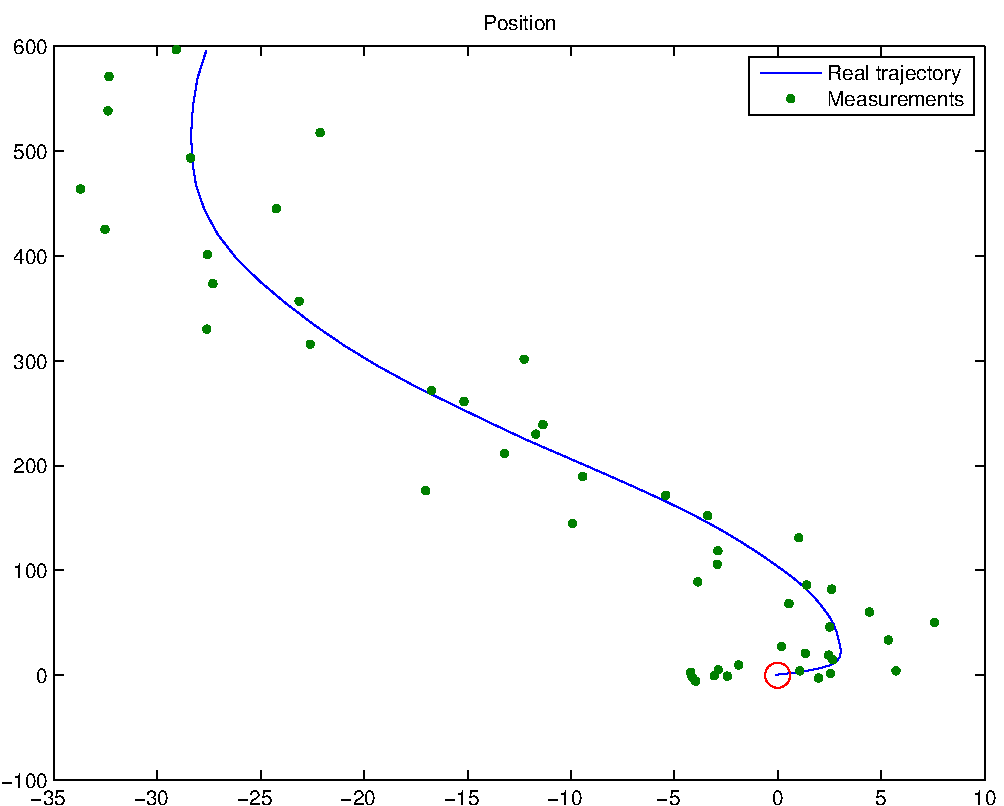
\includegraphics[width=0.7\textwidth]{pics/demo1_f1}
\caption{The real position of the moving object and the simulated
  measurements of it using the CWPA model. The circle marks the
  starting point of the object.}
\label{fig:example1_1}
\end{center}
\end{figure}

The filtering is done with the following code fragment:
%
\begin{lstlisting}
MM = zeros(size(m,1), size(Y,2));
PP = zeros(size(m,1), size(m,1), size(Y,2));

for i = 1:size(Y,2)
   [m,P] = kf_predict(m,P,A,Q);
   [m,P] = kf_update(m,P,Y(:,i),H,R);
   MM(:,i) = m;
   PP(:,:,i) = P;
end
\end{lstlisting}
%
In the first 2 lines the space for state mean and covariance estimates is
reserved, and the rest of the code contains the actual filtering loop, where
we make the predict and update steps of the Kalman filter. The variables
\texttt{m} and \texttt{P} are assumed to contain the initial guesses for the
state mean and covariance before reaching the for-statement. Variable
\texttt{Y} is assumed to contain the measurements made from the system
(See the full source code of the example (\texttt{kf\_cwpa\_demo.m}) provided with the toolbox
to see how we generated the measurements by simulating the dynamic system). In
the end of each iteration the acquired estimates are stored to matrices
\texttt{MM} and \texttt{PP}, for which we reserved space earlier. The estimates
for object's position and velocity with Kalman filter and are plotted in figure
\ref{fig:example1_2}.\\

%\begin{figure}
%\begin{center}
%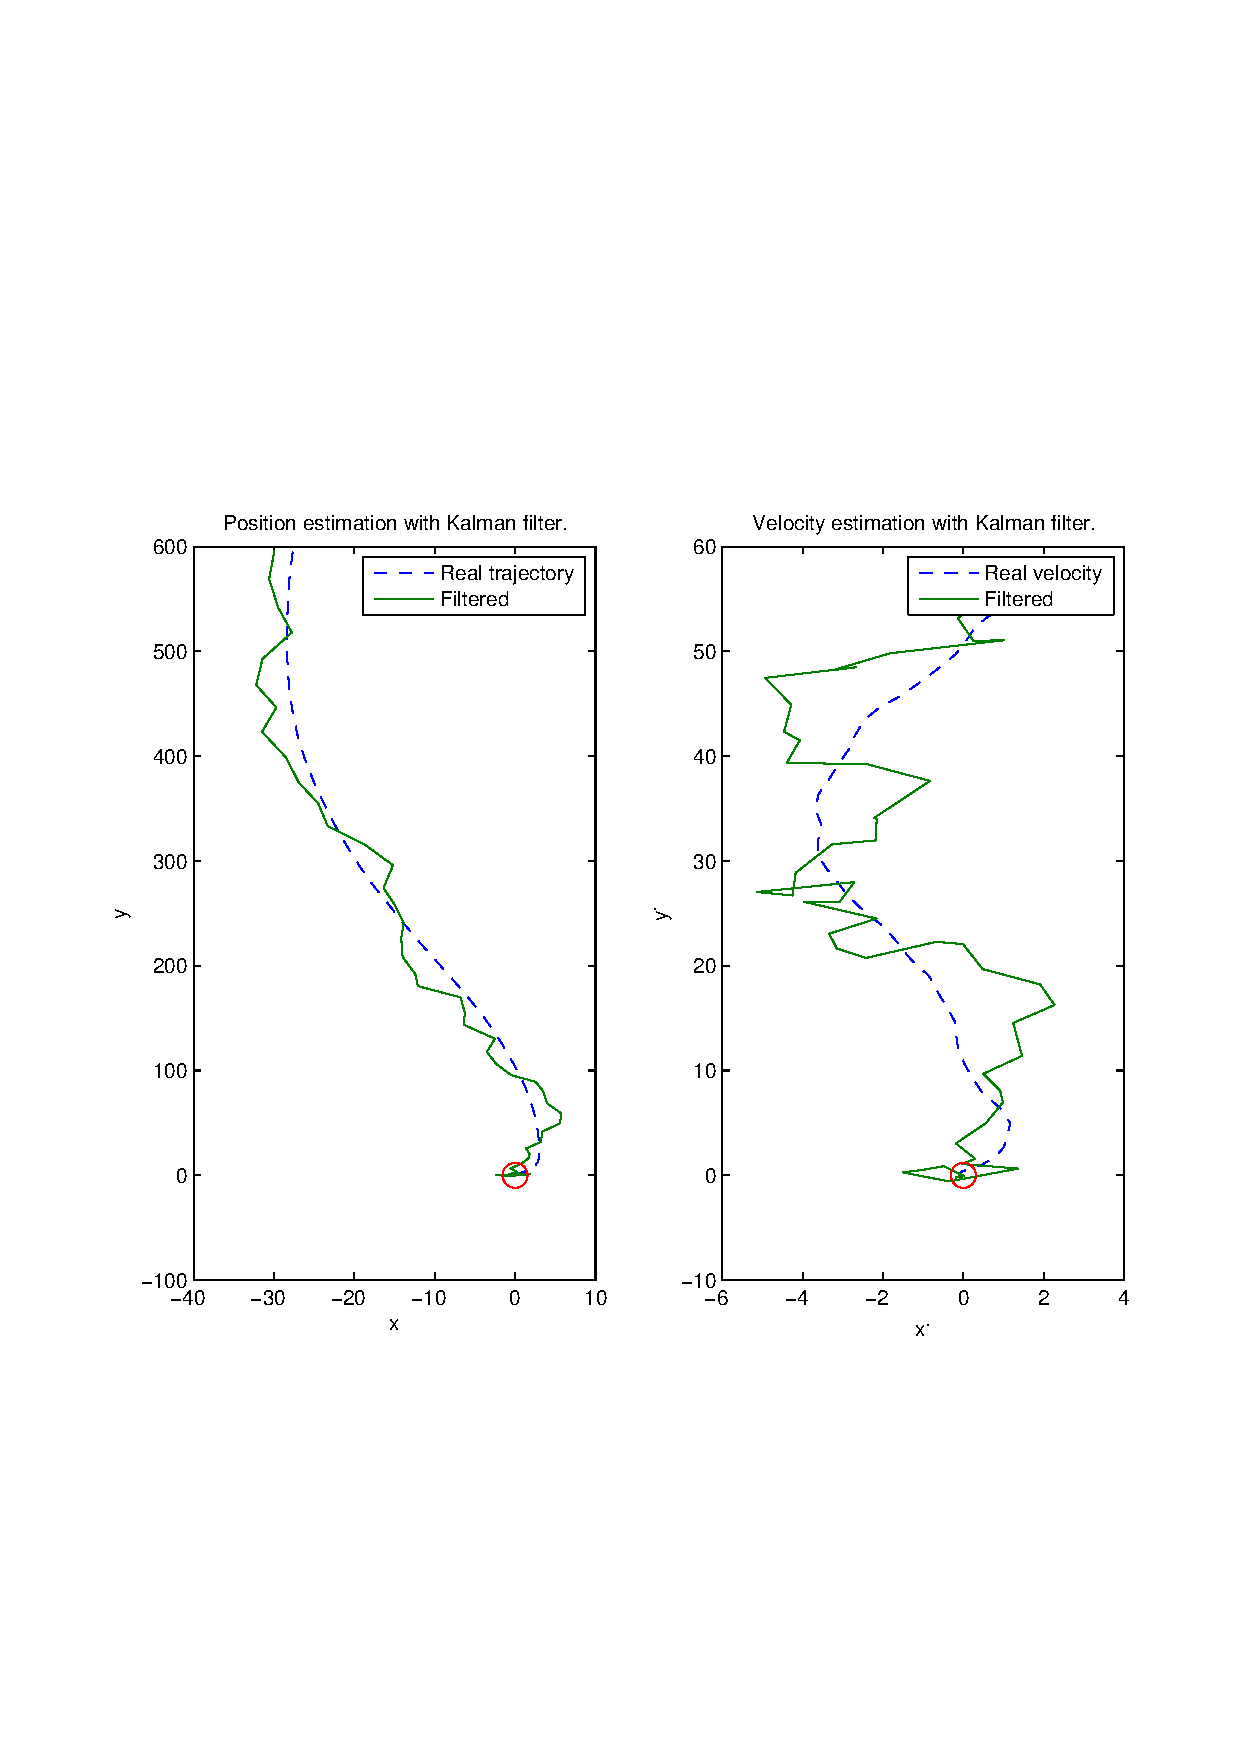
\includegraphics[width=11cm]{pics/demo1_f2}
%\caption{Estimates for position and velocity of the moving object
%  using the Kalman filter and CWPA model.}
%\label{fig:example1_2}
%\end{center}
%\end{figure}

The smoothed estimates for the state mean and covariance can be calculated with the
following code line:
%
\begin{lstlisting}
[SM,SP] = rts_smooth(MM,PP,A,Q);
\end{lstlisting}
%
The calculated smoothed estimates for object's position and velocity for the
earlier demonstration are plotted in figure \ref{fig:example1_3}. As expected
the smoother produces more accurate estimates than the filter as it uses all
measurements for the estimation each time step. Note that the difference between
the smoothed and filtered estimated would be smaller, if the measurements were
more accurate, as now the filter performs rather badly due to the great
uncertaintity in the measurements. The smoothing results of a
forward-backward smoother are not plotted here, as the result are
exactly the same as with the RTS smoother. 

As one would expect the estimates for object's velocity are clearly less
accurate than the estimates for the object's position as the positions are
observed directly and the velocities only indirectly. If the
velocities were also observed not only the velocity estimates would get
more accurate, but also the position ones as well. 

%\begin{figure}
%\begin{center}
%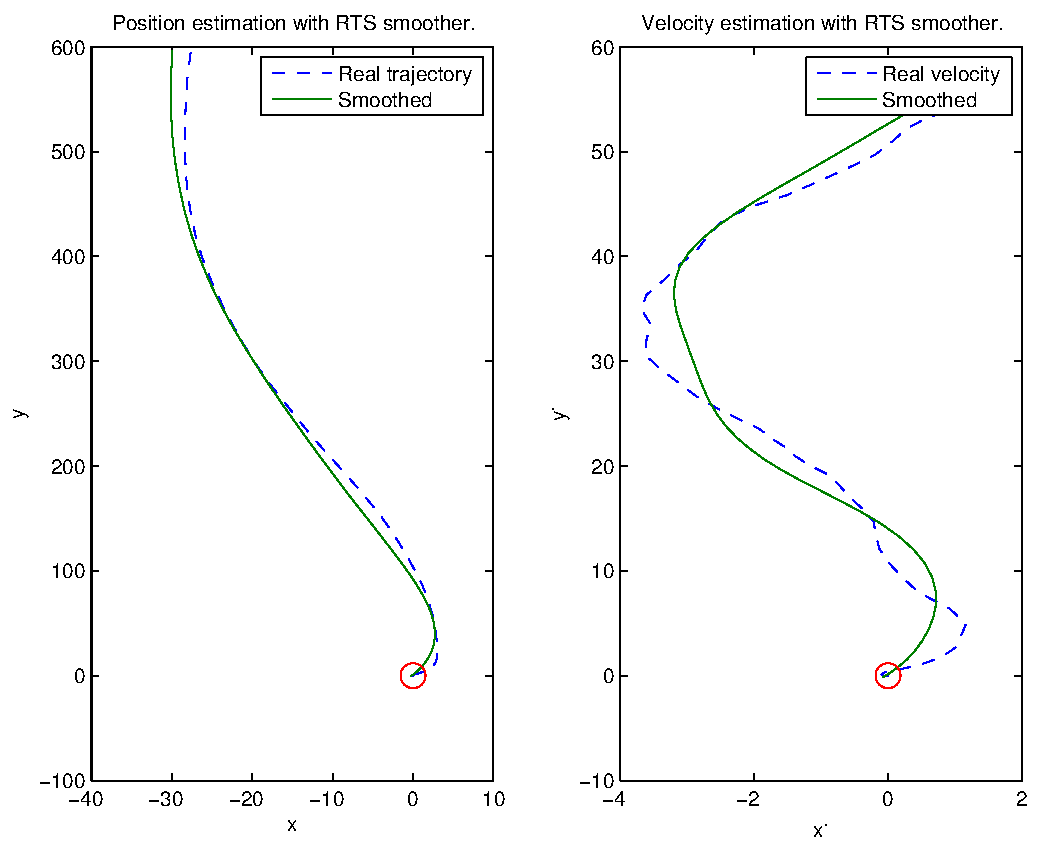
\includegraphics[width=11cm]{pics/demo1_f3}
%\caption{Estimate for position and velocity of the moving object using the RTS smoother and CWPA model.}
%\label{fig:example1_3}
%\end{center}
%\end{figure}




\begin{figure}[t]
 \centering
 \subfigure[Filter]{\label{fig:example1_2}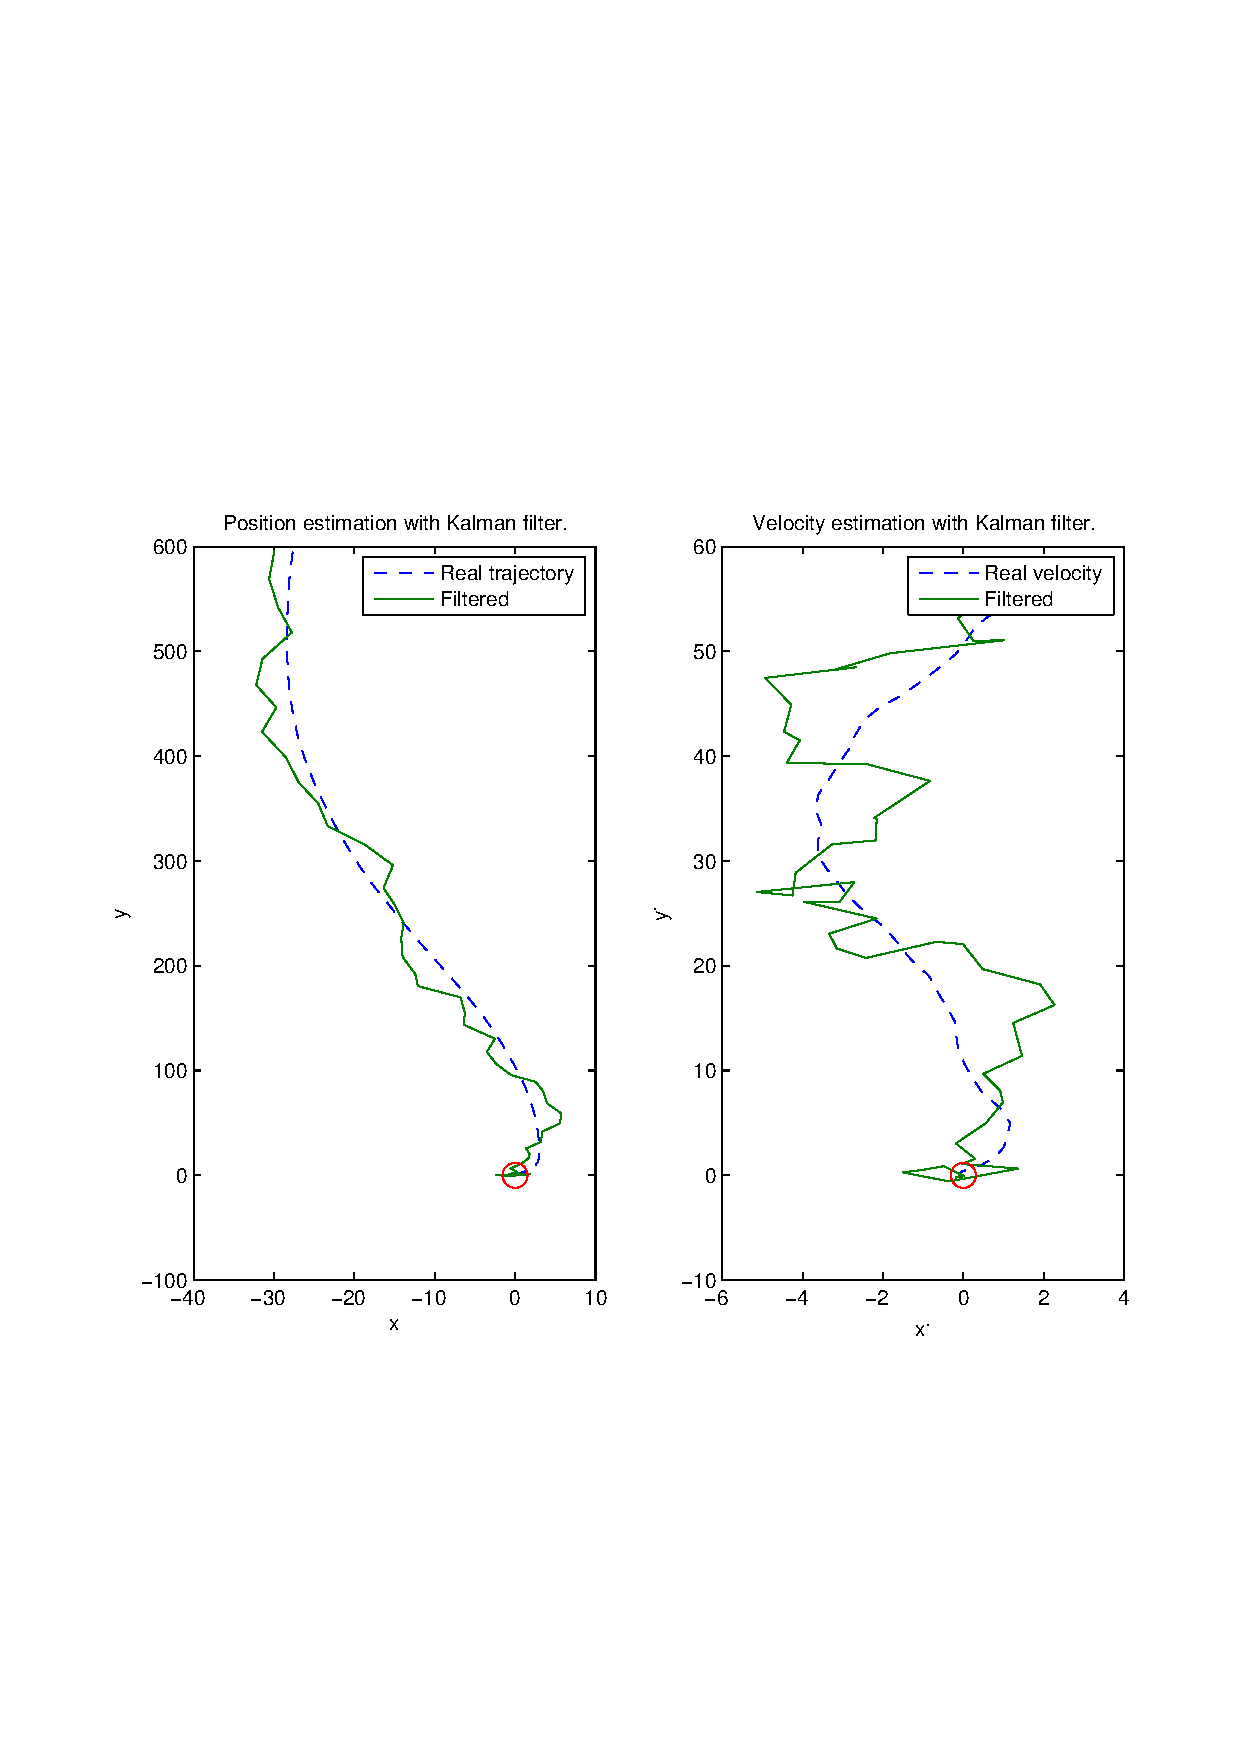
\includegraphics[width=5.5cm]{pics/demo1_f2}}
 \hspace{0.2cm}
 \subfigure[Smoother]{\label{fig:example1_3}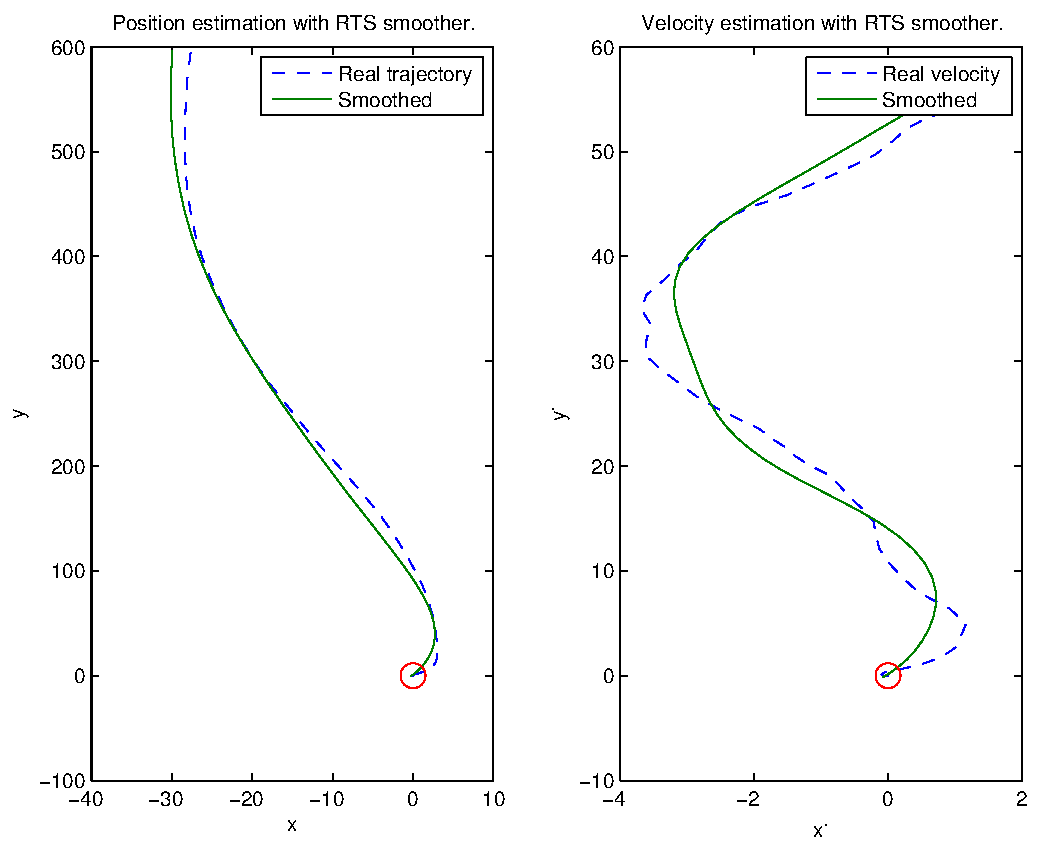
\includegraphics[width=5.5cm]{pics/demo1_f3}}
 %
 \caption{(a) Estimates for position and velocity of the moving object
  using the Kalman filter and CWPA model, and (b) Estimate for position and velocity of the moving object using the RTS smoother and CWPA model.}
 \label{fig:example1_2-3}
\end{figure}









